\documentclass[dvipdfmx,a4paper,11pt]{article}
\usepackage[utf8]{inputenc}
%\usepackage[dvipdfmx]{hyperref} %リンクを有効にする
\usepackage{url} %同上
\usepackage{amsmath,amssymb} %もちろん
\usepackage{amsfonts,amsthm,mathtools} %もちろん
\usepackage{braket,physics} %あると便利なやつ
\usepackage{bm} %ラプラシアンで使った
\usepackage[top=30truemm,bottom=30truemm,left=25truemm,right=25truemm]{geometry} %余白設定
\usepackage{latexsym} %ごくたまに必要になる
\renewcommand{\kanjifamilydefault}{\gtdefault}
\usepackage{otf} %宗教上の理由でmin10が嫌いなので


\usepackage[all]{xy}
\usepackage{amsthm,amsmath,amssymb,comment}
\usepackage{amsmath}    % \UTF{00E6}\UTF{0095}°\UTF{00E5}\UTF{00AD}\UTF{00A6}\UTF{00E7}\UTF{0094}¨
\usepackage{amssymb}  
\usepackage{color}
\usepackage{amscd}
\usepackage{amsthm}  
\usepackage{wrapfig}
\usepackage{comment}	
\usepackage{graphicx}
\usepackage{setspace}
\setstretch{1.2}


\newcommand{\R}{\mathbb{R}}
\newcommand{\Z}{\mathbb{Z}}
\newcommand{\N}{\mathbb{N}}
\newcommand{\C}{\mathbb{C}} 
\newcommand{\Area}{\text{Area}}
\newcommand{\vol}{\text{Vol}}




   %当然のようにやる.
\allowdisplaybreaks[4]
   %もちろん.
%\title{第1回. 多変数の連続写像 (岩井雅崇, 2020/10/06)}
%\author{岩井雅崇}
%\date{2020/10/06}
%ここまで今回の記事関係ない
\usepackage{tcolorbox}
\tcbuselibrary{breakable, skins, theorems}

\theoremstyle{definition}
\newtheorem{thm}{定理}
\newtheorem{lem}[thm]{補題}
\newtheorem{prop}[thm]{命題}
\newtheorem{cor}[thm]{系}
\newtheorem{claim}[thm]{主張}
\newtheorem{dfn}[thm]{定義}
\newtheorem{rem}[thm]{注意}
\newtheorem{exa}[thm]{例}
\newtheorem{conj}[thm]{予想}
\newtheorem{prob}[thm]{問題}
\newtheorem{rema}[thm]{補足}

\DeclareMathOperator{\Ric}{Ric}
\DeclareMathOperator{\Vol}{Vol}
 \newcommand{\pdrv}[2]{\frac{\partial #1}{\partial #2}}
 \newcommand{\drv}[2]{\frac{d #1}{d#2}}
  \newcommand{\ppdrv}[3]{\frac{\partial #1}{\partial #2 \partial #3}}


%ここから本文.
\begin{document}
%\maketitle
\begin{center}
{\Large 第9回. 可測性と可積分性 (川平先生の本, 第25章の内容)}
\end{center}

\begin{flushright}
 岩井雅崇, 2020/12/08
\end{flushright}
 \section{はじめに}
 この回の内容はかなり難しいので, 積分の理論を気にせず計算だけしたい人はこの回の内容を読み飛ばして, 次の回の内容に移って良い.
 (最後の誤差評価は使えるかもしれませんが...)
 
 また証明等を少々省略するので, 詳しくリーマン積分を理解したい人は次の文献を見てほしい.
 \begin{itemize}
 \item 杉浦光夫 解析入門 1 (東京大学出版会)
 \end{itemize}
 
動画冒頭に述べたルベーグ積分を理解したい人は次の文献を見てほしい.
(めちゃくちゃ難しいですが...)
 \begin{itemize}
 \item 伊藤清三 ルベーグ積分入門 (裳華房)
 \item Terence Tao \textit{An introduction to measure theory}
 available at \url{https://terrytao.files.wordpress.com/2011/01/measure-book1.pdf}
 \end{itemize}
 
リーマン積分もルベーグ積分もどちらも計算上は違いはないので, 積分の理論を気にせず, 計算だけしたい場合は気にしなくて良いです.

\section{リーマン積分の定義}
この節では
$D = [a,b]\times [c,d] = \{ (x,y) \in \R^2 : a \leqq x \leqq b, c \leqq y \leqq d\}%\text{\,\,とする.}$
$とする.
 \begin{itemize}
 \item \underline{関数$f(x,y)$が$D$上で有界}であるとは, ある正の数$M>0$があって, 任意の$(x,y)\in D$について$|f(x,y) |<M$となること.
 
\hspace{-22pt} 以下, 関数$f(x,y)$が$D$上で有界であるとする.
 \item \underline{$\Delta$が$D$の分割}とは, ある正の自然数$m,n$と
 $$
 a = x_{0}<x_1< \dots , x_{m-1}<x_{m}=b, \text{\,\,\,}
c = y_{0}<y_1< \dots , y_{n-1}<y_{n}=d, \text{\,\,となる}
 $$
 数の組$( a, x_1, \dots , x_{m-1} , b), ( c, y_1, \dots , y_{n-1} , d)$のこと.
 
 以下$\Delta = \{ ( a, x_1, \dots , x_{m-1} , b ),( c, y_1, \dots , y_{n-1} , d )\}$とかく. (この授業だけの記号である.)
 \item $\Delta$を$D$の分割として, \underline{$\Delta$の長さ}を
 $$
| \Delta| = \max_{1 \leqq i \leqq m, 1 \leqq j \leqq n} \{ |x_i - x_{i-1}|, |y_{j} - y_{j-1}|\} 
 \text{\,\,とする.}
 $$
 
 \item $\Delta$を$D$の分割とする.
 $1 \leqq i \leqq m, 1 \leqq j \leqq n$となる自然数$i,j$について
 $$
 M_{ij} = \max \{ f(x,y) :x_{i-1} \leqq x \leqq x_i , y_{j-1} \leqq y \leqq y_{j} \},
 $$
 $$
 m_{ij} = \min \{ f(x,y) : x_{i-1} \leqq x \leqq x_i , y_{j-1} \leqq y \leqq y_{j} \} \text{\,\,とし, }
 \footnote{最大値最小値の存在は自明ではないので実は間違い. 本当は上限(sup)と下限(inf)を用いて
 $$
  M_{ij} = \sup \{ f(x,y) : x_{i-1} \leqq x \leqq x_i , y_{j-1} \leqq y \leqq y_{j} \}, \text{\,\,}
 m_{ij} = \inf \{ f(x,y) : x_{i-1} \leqq x \leqq x_i , y_{j-1} \leqq y \leqq y_{j} \} 
 $$
 と書く. (おそらく上限や下限を習ってないと思うので, 今回はmax, minで定義します.)}
 $$
 
  
 $$
 S_{\Delta} = \sum_{j=1}^{n}\sum_{i=1}^{m} M_{ij}(x_i - x_{i-1})(y_{j} - y_{j-1}), \text{\,\,\,\,}
  T_{\Delta} = \sum_{j=1}^{n}\sum_{i=1}^{m} m_{ij}(x_i - x_{i-1})(y_{j} - y_{j-1})\text{\,\,とおく. }
 $$
定義から$T_{\Delta} \leqq S_{\Delta}$となる.

 \end{itemize}
 
  \begin{tcolorbox}[
    colback = white,
    colframe = green!35!black,
    fonttitle = \bfseries,
    breakable = true]
    \begin{thm}[ダルブーの定理]
    ある実数$S,T$があって, 
    $$
    \lim_{|\Delta| \rightarrow 0}S_{\Delta} = S, \text{\,\,} \lim_{|\Delta| \rightarrow 0}T_{\Delta} = T.
    $$
    \end{thm}
    \end{tcolorbox}
    \footnote{$\lim_{|\Delta| \rightarrow 0}S_{\Delta} = S$の意味は, $\Delta$の長さが0になるように分割をとっていくと, $S_{\Delta}$は$S$に限りなく近くという意味である.}
    
      \begin{tcolorbox}[
    colback = white,
    colframe = green!35!black,
    fonttitle = \bfseries,
    breakable = true]
    \begin{dfn}
    $D = [a,b]\times [c,d]$かつ$f(x,y)$を$D$上の有界関数とする. \\
    \underline{$f$が$D$上でリーマン積分可能(リーマン可積分)}とは$S=T$となること.
    このとき, 
    $$
    S = \iint_{D} f(x,y)dxdy \text{\,\,と表す.}
    $$
    \underline{$S$を$f(x,y)$の$D$上での重積分}といい, \underline{$D$を積分領域}, \underline{$f$を被積分関数}という.
    \end{dfn}
    \end{tcolorbox}
    以下, リーマン積分可能を単に積分可能ということにする.

\begin{exa}
\label{riem_not}
\begin{itemize}
\item $D = [a,b]\times [c,d]$とし, $f$を$D$上での連続関数とする.
このとき$f$は$D$上で積分可能.(みんながよく知っている関数は積分可能.)
\item $D = [0,1]\times[0,1]$とし, $D$上の有界関数$f(x,y)$を
$$
  f(x,y)= \begin{cases}
     1& \text{$x$も$y$も共に有理数}\\
    0& \text{上以外}
  \end{cases}
$$
とおくとき, 任意の$D$の分割$\Delta$について, $S_{\Delta}=1$であり, $T_{\Delta}=0$である.
よって$S =1$かつ$T=0$より, $f$は$D$上で積分可能ではない.
\footnote{ルベーグ積分は可能になる. 積分値は0となる. ルベーグ積分はいい感じにリーマン積分を包含する概念である.}
 \end{itemize}
\end{exa}

\section{一般集合上での積分}
      \begin{tcolorbox}[
    colback = white,
    colframe = green!35!black,
    fonttitle = \bfseries,
    breakable = true]
    \begin{dfn}
    $D \subset \R^2$を有界集合とし, ある正の数$M>0$を$D \subset [-M,M]\times[-M,M]$となるようにとる.
    $\tilde{D} = [-M,M]\times[-M,M]$とおく.
    
    $f(x,y)$を$D$上の有界関数として, \underline{$f$が$D$上リーマン積分可能(リーマン可積分)}
    とは
    $$
  \tilde{f}(x,y)= \begin{cases}
     f(x,y)& (x,y) \in D\\
    0& (x,y) \not \in D
  \end{cases}
$$
とおくとき, $\tilde{f}$が$\tilde{D}$上で積分可能であること.
    このとき
    $$
    \iint_{D}f(x,y)dxdy = \iint_{\tilde{D}} \tilde{f}(x,y)dxdy \text{\,\,と定義する.}
    $$
    \end{dfn}
    \end{tcolorbox}

      \begin{tcolorbox}[
    colback = white,
    colframe = green!35!black,
    fonttitle = \bfseries,
    breakable = true]
    \begin{dfn}

    $D \subset \R^2$を有界集合とする.
    \underline{$D$が面積確定(ジョルダン可測)}とは$D$上の定数関数$f(x,y)=1$が$D$上で(リーマン)積分可能であること. 
このとき
$$
\Area(D) = \iint_{D} dxdy = \iint_{D} 1 dxdy \text{\,\,と表す.}
$$
        \end{dfn}
    \end{tcolorbox}
    
\begin{exa}

\begin{itemize}
\item $D=[a,b]\times [c,d]$とすると$D$は面積確定である. 面積$\Area(D)=(b-a)(d-c)$である.
\item $\phi_1(x), \phi_{2}(x)$を$\phi_1(x) \leqq \phi_2(x)$となる$[a,b]$上の連続関数とする. \\ $
D = \{ (x,y) \in \R^2 : a \leqq x \leqq b, \phi_1(x) \leqq y \leqq \phi_2(x)\}
$
とおくとき, $D$は面積確定で, 
$$\Area(D) = \int_{a}^{b} \{ \phi_2(x) - \phi_1(x)\}dx \text{\,\,となる.}\footnote{第10回の資料によりわかる.}$$

特に半径1の円は
$
D = \{ (x,y) \in \R^2 :\ -1 \leqq x \leqq 1, -\sqrt{1-x^2} \leqq y \leqq \sqrt{1-x^2} \}
$
と書けるので, $\Area(D) = \pi$となる.\footnote{これも第10回の資料によりわかる.}
(みんながよく知っている図形は面積確定.)
\item $D = \{ (x,y) \in \R^2 : \text{$x$も$y$も共に有理数}\}$とおくとき,  例\ref{riem_not}から$D$は面積確定ではない.
\end{itemize}
\end{exa}

      \begin{tcolorbox}[
    colback = white,
    colframe = green!35!black,
    fonttitle = \bfseries,
    breakable = true]
    \begin{thm}
$D$を面積確定な有界閉集合とし, $f$を$D$上で連続とするとき, $f$は$D$上で積分可能である.
        \end{thm}
    \end{tcolorbox}
 以上から, みんながよく知っている図形の上での, みんながよく知っている関数の積分は可能である.
    
\section{重積分の性質.}
      \begin{tcolorbox}[
    colback = white,
    colframe = green!35!black,
    fonttitle = \bfseries,
    breakable = true]
    \begin{prop}
$D, D_1,D_2$を面積確定な有界閉集合とし, 
$f(x,y), g(x,y)$を連続関数とする.
\begin{enumerate}
\item \text{$\Area(D_1 \cap D_2)=0$ならば}
$$
\iint_{D_1 \cup D_2}fdxdy = \iint _{D_1}fdxdy +\iint _{D_2}fdxdy.
$$
\item $D$上$f(x,y) \leqq g(x,y)$のとき, 
$$
\iint _{D}fdxdy  \leqq \iint_{D} gdxdy.
$$

\item $\alpha$を実数とするとき, 
$$
\iint _{D}\{f +g\}dxdy = \iint _{D}fdxdy + \iint _{D}gdxdy, \text{\,\,}
 \iint _{D}\alpha fdxdy = \alpha  \iint _{D}fdxdy.
$$

\item ある実数$M>0$があって, $D$上で$|f(x,y)| \leqq M$のとき, 
$$
\iint _{D}fdxdy  \leqq M \Area(D).
$$
\end{enumerate}

        \end{prop}
    \end{tcolorbox}

\section{数値積分の精度}

      \begin{tcolorbox}[
    colback = white,
    colframe = green!35!black,
    fonttitle = \bfseries,
    breakable = true]
    \begin{thm}
$D=[a,b] \times [c,d]$とし, 
$f$を$D$上の$C^1$級関数とする. \\
$\max_{(x,y)\in D} \left\{ |\pdrv{f}{x}(x,y)|, |\pdrv{f}{y}(x,y)| \right\} \leqq K_1$となる実数$K_1$をとる.

$\Delta$を$D$の分割とすると, 
$$
(S_{\Delta} -T_{\Delta} )\leqq 2K_1 \Area(D) |\Delta| = 2K_{1}(b-a)(d-c)  |\Delta|  \text{\,\,となる.}
$$
        \end{thm}
    \end{tcolorbox}

      \begin{tcolorbox}[
    colback = white,
    colframe = green!35!black,
    fonttitle = \bfseries,
    breakable = true]
    \begin{thm}[区分求積法]
$D=[a,b] \times [c,d]$とし, 
$f$を$D$上の$C^1$級関数, $N>0$を正の自然数とする. 
$\max_{(x,y)\in D} \left\{ |\pdrv{f}{x}(x,y)|, |\pdrv{f}{y}(x,y)| \right\} \leqq K_1$となる実数$K_1$をとる.
$$
I = \iint_{D} f dxdy, \text{\,\,\,\,} 
\Sigma_N=\sum_{j=1}^{N}\sum_{i=1}^{N}f\left(  a+i\frac{(b-a)}{N} ,c+j\frac{(d-c)}{N}\right)\frac{(b-a)(d-c)}{N^2}
\text{とおくとき,}
$$
$$
|I-\Sigma_{N}| \leqq \frac{K_1(b-a)(d-c)\{ b-a+d-c\}}{N}.
$$
とくに
$\lim_{N \rightarrow \infty} \Sigma_{N} = I $
となる.
        \end{thm}
    \end{tcolorbox}
\begin{exa}
$D=[0,1]\times [0,1]$とし, $f(x,y)=x^2+y^2$とする.
$$
\max_{(x,y)\in D} \left\{ |\pdrv{f}{x}(x,y)|, |\pdrv{f}{y}(x,y)| \right\} 
=
\max_{(x,y)\in D} \left\{ |2x|, |2y| \right\} 
=
2
$$
より, $K_1=2$と取れる.

$N$を正の自然数とすると, 
$I = \iint_{D} f dxdy, =\frac{2}{3}$, $\frac{K_1(b-a)(d-c)\{ b-a+d-c\}}{N}=\frac{4}{N}$,
$$\Sigma_{N}=
\sum_{j=1}^{N}\sum_{i=1}^{N}f\left( \frac{i}{N},\frac{j}{N}\right)
=\sum_{j=1}^{N}\sum_{i=1}^{N}\frac{i^2+j^2}{N^4} \text{\,\,であるので. }
|I - \Sigma_{N}|=\left|\frac{2}{3} - \sum_{j=1}^{N}\sum_{i=1}^{N}\frac{i^2+j^2}{N^4} \right| \leqq \frac{4}{N}.
$$
\end{exa}

\newpage

\begin{center}
{\Large 第10回. 累次積分 (川平先生の本, 第26章の内容)}
\end{center}

\begin{flushright}
 岩井雅崇, 2020/12/15
\end{flushright}
 
 \section{縦線領域と累次積分}
 
 \begin{tcolorbox}[
    colback = white,
    colframe = green!35!black,
    fonttitle = \bfseries,
    breakable = true]
    \begin{dfn}
   $\phi_1(x), \phi_{2}(x)$を$\phi_1(x) \leqq \phi_2(x)$となる$[a,b]$上の連続関数とする. 
   $$
D = \{ (x,y) \in \R^2 : a \leqq x \leqq b, \phi_1(x) \leqq y \leqq \phi_2(x)\}
$$
で表せられる領域を\underline{縦線領域}という.
 \end{dfn}
 \end{tcolorbox}
 
 
 
 \begin{exa}

\begin{itemize}
\item $D=[a,b]\times [c,d]$は縦線領域. $\phi_1(x)=c$, $\phi_2(x)=d$とすれば良い.
\item 縦線領域
$D = \{ (x,y) \in \R^2 :\ -1 \leqq x \leqq 1, -\sqrt{1-x^2} \leqq y \leqq \sqrt{1-x^2} \}$
とおくと$D$は原点中心の半径1の円.
\end{itemize}
\end{exa}
 
 \begin{tcolorbox}[
    colback = white,
    colframe = green!35!black,
    fonttitle = \bfseries,
    breakable = true]
    \begin{thm}
縦線領域を$D = \{ (x,y) \in \R^2 : a \leqq x \leqq b, \phi_1(x) \leqq y \leqq \phi_2(x)\}$とし, $f(x,y)$
を$D$上の連続関数とする.
このとき, $f(x,y)$は$D$上で積分可能であり,
$$
\iint_{D} f(x,y)dxdy = \int_{a}^{b }\left( \int_{\phi_1(x)}^{\phi_{2}(x)}f(x,y)dy    \right) dx \text{\,\,となる.}
$$
これを\underline{$f(x,y)$の累次積分}という.

特に$D$は面積確定で
$$
\Area(D) = \iint_{D} dxdy=\int_{a}^{b} \{ \phi_2(x) - \phi_1(x)\}dx.
$$
        \end{thm}
 \end{tcolorbox}
 
  \begin{exa}
 $D=[0,1]\times[0,1]$, $f(x,y)=x^2+y^2$とする.
 $\iint_{D}f(x,y)dxdy$を求めよ.

\hspace{-11pt}(解.) $\phi_1(x)=0, \phi_2(x)=1$とすると上の定理より, 

$$
%  \iint_{D}f(x,y)dxdy %&=  \int_{0}^{1}\left( \int_{0}^{1} x^2+y^2dy    \right) dx \\ &
\iint_{D}x^2+y^2dxdy 
  =  \int_{0}^{1}\left( \int_{0}^{1} x^2+y^2dy    \right) dx 
  = \int_{0}^{1}\left[ x^{2}y + \frac{y^3}{3}   \right]_{0}^{1} dx 
  =\int_{0}^{1} x^{2}+ \frac{1}{3}  dx 
  =\left[  \frac{x^3}{3} +\frac{x}{3}  \right]_{0}^{1} =\frac{2}{3}.
$$
 \end{exa}
 
   \begin{exa}
$D = \{ (x,y) \in \R^2 : -1 \leqq x \leqq 1, -\sqrt{1-x^2} \leqq y \leqq \sqrt{1-x^2} \}$とする.
$\Area(D) = \iint_{D} dxdy$を求めよ.

\hspace{-11pt}(解.) $\phi_1(x)=-\sqrt{1-x^2}, \phi_2(x)=\sqrt{1-x^2} $とすると上の定理より, 

$$
  \iint_{D}dxdy =\int_{-1}^{1} \left\{ \sqrt{1-x^2} - \left(-\sqrt{1-x^2} \right) \right\} dx
  = 2 \int_{-1}^{1} \sqrt{1-x^2} dx =\pi.
$$
  \end{exa}
つまり半径1の円の面積は$\pi$.
 
    \begin{exa}
$D = \{ (x,y) \in \R^2 : 0 \leqq x \leqq 1, x^2 \leqq y \leqq 1 \}$とし, 
$f(x,y)=xe^{-y^2}$とするとき,  $\iint_{D}f(x,y)dxdy$を求めよ.

\hspace{-11pt}(解.) 普通に定理を適用すると, 
$$
\iint_{D} xe^{-y^2}dxdy = \int_{0}^{1} \left( \int_{x^2}^{1} xe^{-y^2}dy    \right) dx
$$
となるが, $e^{-y^2}$の不定積分がわからないため, ここで手詰まりとなる.

そこで$D = \{ (x,y) \in \R^2 : 0 \leqq y \leqq 1, 0 \leqq x \leqq \sqrt{y} \}$に注意すると, 
\begin{align*}
\begin{split}
\iint_{D} xe^{-y^2}dxdy &= \int_{0}^{1} \left( \int_{0}^{\sqrt{y}} xe^{-y^2}dx   \right) dy \\
&= \int_{0}^{1}\left[ \frac{x^{2} e^{-y^2} }{2}  \right]_{0}^{\sqrt{y}} dy
=  \int_{0}^{1}    \frac{y e^{-y^2} }{2}      dy
= \left[  \frac{- e^{-y^2} }{4}   \right]_{0}^{1} = \frac{1}{4}\left( 1 - \frac{1}{e}\right).
\end{split}
\end{align*}

  \end{exa}
\newpage

\begin{center}
{\Large 第11回. 多重積分の変数変換公式 (川平先生の本, 第27章の内容)}
\end{center}

\begin{flushright}
 岩井雅崇, 2020/12/22
\end{flushright}


\section{変数変換公式}
 \begin{tcolorbox}[
    colback = white,
    colframe = green!35!black,
    fonttitle = \bfseries,
    breakable = true]
    \begin{dfn}
 $E \subset \R^2$を集合とする. 
 \underline{点$(a,b) \in \R^2$が$E$の境界}であるとは. 任意の正の数$r>0$について
 $B_{(a,b)}(r) = \{ (x,y)\in \R^2 :\sqrt{(x-a)^2 + (y-b)^2 } \leqq r  \}$とするとき, 
 $B_{(a,b)}(r) \cap E \neq \phi$かつ$B_{(a,b)}(r) \cap (\R^2 \setminus E) \neq \phi$となること.
\underline{ $E$の境界の点からなる集合を$\partial E$}とする.
 \end{dfn}
 \end{tcolorbox}
 \footnote{ $B_{(a,b)}(r) \cap E \neq \phi$ とは$B_{(a,b)}(r) \cap E$が空集合でないこと. つまり, ある元$(c,d) \in B_{(a,b)}(r) \cap E $が存在すること.}
 
 \begin{exa}
 $E = \{ (x,y)\in \R^2 :\sqrt{x^2 + y^2 } \leqq 1  \}$とする.このとき$E$の境界の点の集合は
 $$
 \partial E = \{ (x,y)\in \R^2 :\sqrt{x^2 + y^2 } = 1  \} \text{\,\,となる.}
 $$
 \end{exa}

 \begin{tcolorbox}[
    colback = white,
    colframe = green!35!black,
    fonttitle = \bfseries,
    breakable = true]
    \begin{dfn}
$E \subset \R^2$を面積確定な有界閉集合とし, 変数変換$\Phi$を次の通りとする.

 $$
\begin{array}{ccccc}
\Phi: &E & \rightarrow & \R^2 & \\
&(u,v) & \longmapsto & (x(u,v),y(u,v))&
\end{array}
$$

\underline{$\Phi$が重積分の変数変換の条件を満たす}とは, 次の条件(1)-(3)を満たすこと.

[条件(1).] $x(u,v),y(u,v)$は$C^1$級である.

[条件(2).] $D = \Phi(E)$とするとき, $E$の境界以外で$\Phi$は1対1写像. 

[条件(3).] $\Phi$のヤコビ行列
$$
D\Phi=
\left(\begin{array}{cc} \pdrv{x}{u} & \pdrv{x}{v} \\ \pdrv{y}{u}& \pdrv{y}{v} \\ \end{array} \right)
$$ 
とし, ヤコビアンを$\det D\Phi = 
\Bigl( \pdrv{x}{u} \Bigr) \left( \pdrv{y}{v} \right) - \Bigl( \pdrv{x}{v}  \Bigr) \left( \pdrv{y}{u}\right)$とするとき, $\det D\Phi $は$E$の境界以外で0にならない.
 \end{dfn}
 \end{tcolorbox}

\begin{exa}
\begin{itemize}
\item $E=[0,1]\times[0,1]$とし, 
 $$
\begin{array}{ccccc}
\Phi: &E & \rightarrow & \R^2 & \\
&(u,v) & \longmapsto & (u+v,v)&
\end{array}
$$
とすると, 条件(1)-(3)を満たす.
特に$
D\Phi=
\left(\begin{array}{cc} 1 &1 \\ 0& 1 \\ \end{array} \right)
$
かつ$\det D\Phi =1 \neq 0$である.

\item $E=[0,1]\times[0,1]$とし, 
 $$
\begin{array}{ccccc}
\Phi: &E & \rightarrow & \R^2 & \\
&(u,v) & \longmapsto & (u+v,u+v)&
\end{array}
$$
とすると, 条件(3)を満たさない.
実際$
D\Phi=
\left(\begin{array}{cc} 1 &1 \\ 1& 1 \\ \end{array} \right)
$
かつ$\det D\Phi =0$である.

\item $E=[0,1]\times[0,2\pi]$とし, 
 $$
\begin{array}{ccccc}
\Phi: &E & \rightarrow & \R^2 & \\
&(r,\theta) & \longmapsto & (r \cos \theta , r \sin \theta)&
\end{array}
$$
とすると, 条件(1)-(3)を満たし. $D = \Phi(E) =  \{ (x,y)\in \R^2 :\sqrt{x^2 + y^2 } \leqq 1  \}$となる.
特に$
D\Phi=
\left(\begin{array}{cc} \cos \theta  &-r \sin \theta \\ \sin \theta& r \cos \theta  \\ \end{array} \right)
$
かつ$\det D\Phi =r$である.\footnote{この例では$E \setminus \partial E = \{ (r,\theta)\in \R^2 : 0 < r<1, 0<\theta <2\pi\}$であるため, $E$の境界以外の集合である$E \setminus\partial E$上で$\det D\Phi =r$は0ではない.}

\item $E=[0,1]\times[0,4\pi]$とし, 
 $$
\begin{array}{ccccc}
\Phi: &E & \rightarrow & \R^2 & \\
&(r,\theta) & \longmapsto & (r \cos \theta , r \sin \theta)&
\end{array}
$$
とすると, 条件(2)を満たさない.
\footnote{$\Phi(\frac{1}{2}, \pi)=\Phi( \frac{1}{2}, 3\pi) =(-\frac{1}{2}, 0)$であるため1対1ではない. 1対1に関しては第4回授業を参照のこと.}
\end{itemize}

\end{exa}

 \begin{tcolorbox}[
    colback = white,
    colframe = green!35!black,
    fonttitle = \bfseries,
    breakable = true]
    \begin{thm}[多重積分の変数変換公式]
$E \subset \R^2$を面積確定な有界閉集合とし, 変数変換$\Phi$を次の通りとする.

 $$
\begin{array}{ccccc}
\Phi: &E & \rightarrow & \R^2 & \\
&(u,v) & \longmapsto & (x(u,v),y(u,v))&
\end{array}
$$
$\Phi$は重積分の変数変換の条件(条件(1)-(3))を満たすとする.

関数$f(x,y)$が$D = \Phi(E)$上で積分可能であるとき
$$
\iint_{D}f(x,y)dxdy=\iint_{E} f(x(u,v),y(u,v))|\det D \Phi|dudv \text{\,\,となる.}
$$
 \end{thm}
 \end{tcolorbox}

\begin{exa}
$D= \{ (x,y)\in \R^2 :\sqrt{x^2 + y^2 } \leqq 1  \}$とする. 
$\iint_{D} e^{-x^2-y^2}dxdy$を求めよ.

\hspace{-11pt}(解.) 
$E=[0,1]\times[0,2\pi]$とし, 
 $$
\begin{array}{ccccc}
\Phi: &E & \rightarrow & \R^2 & \\
&(r,\theta) & \longmapsto & (r \cos \theta , r \sin \theta)&
\end{array}
$$
とすると, 条件(1)-(3)を満たし. $D = \Phi(E)$かつ$\det D\Phi =r$である.

以上より多重積分の変数変換の公式から
\begin{align*}
\begin{split}
\iint_{D} e^{-x^2-y^2}dxdy
&=
\iint_{E} e^{-(r \cos \theta )^2- (r \sin \theta )^2} |r|drd\theta \\
&=
\iint_{E} e^{-r^2}r drd\theta \\
&=
\int_{0}^{2\pi} \left( \int_{0}^{1}e^{-r^2}r dr\right)d\theta 
=\int_{0}^{2\pi} \left[ \frac{-e^{-r^2}}{2} \right]_{0}^{1} d\theta 
=\int_{0}^{2\pi} \frac{1-e^{-1}}{2} d\theta =\pi\left( 1-\frac{1}{e}\right).
    \end{split}
  \end{align*}
\end{exa}

\begin{exa}
$D= \{ (x,y)\in \R^2 : |x+2y|\leqq1, |x-y|\leqq1 \}$とする. 
$\iint_{D} (x-y)^2dxdy$を求めよ.

\hspace{-11pt}(解.) 
$E=[-1,1]\times[-1,1]$とし, 
 $$
\begin{array}{ccccc}
\Phi: &E & \rightarrow & \R^2 & \\
&(u,v) & \longmapsto & (\frac{u+2v}{3} , \frac{u-v}{3} )&
\end{array}
$$
とすると, 条件(1)-(3)を満たし, 
$D = \Phi(E)$かつ$
D\Phi=
\left(\begin{array}{cc} \frac{1}{3} &\frac{2}{3} \\ \frac{1}{3}&-\frac{1}{3} \\ \end{array} \right)
$
かつ$\det D\Phi = -\frac{1}{3}\neq 0$である.
以上より多重積分の変数変換の公式から, 
\begin{align*}
\begin{split}
\iint_{D} (x-y)^2dxdy
&=
\iint_{E} \left(  \frac{u+2v}{3} - \frac{(u-v)}{3} \right)^2 \left| -\frac{1}{3}\right| dudv \\
&= 
\iint_{E} \frac{v^2}{3} dudv
=
\int_{-1}^{1} \left( \int_{-1}^{1} \frac{v^2}{3} dv\right)du 
=
\int_{-1}^{1} \left[ \frac{v^3}{9}\right]_{-1}^{1} du
=\int_{-1}^{1}  \frac{2}{9} du
=\frac{4}{9}. 
 \end{split}
  \end{align*}




\end{exa}
 
 
\newpage


\begin{center}
{\Large 第12回. 広義積分とガンマ関数 (川平先生の本, 第12・27章の内容)}
\end{center}

\begin{flushright}
 岩井雅崇, 2021/01/12
\end{flushright}


\section{広義積分}
この回は1変数の積分に関しても取り扱う.(ガウス積分以外は1変数の積分の話である.)
 \begin{tcolorbox}[
    colback = white,
    colframe = green!35!black,
    fonttitle = \bfseries,
    breakable = true]
    \begin{dfn}
$f(x)$を$[a,b)$上の連続関数とする.($b=+\infty$も許す.)
左極限$\lim_{z \rightarrow b-0} \int_{a}^{z} f(x)dx$が存在するとき, 
\underline{広義積分 $\int_{a}^{b} f(x)dx$は収束する}といい
$$
\int_{a}^{b} f(x)dx = \lim_{z \rightarrow b-0} \int_{a}^{z} f(x)dx \text{\,\,とする.}
$$
この積分を\underline{広義積分}という.
極限が存在しないときは, \underline{$\int_{a}^{b} f(x)dx$は発散する}という.
 \end{dfn}
 \end{tcolorbox}
 
 \begin{exa}
 \begin{itemize}
 \item $\int_{1}^{\infty} x^p dx$は$p<-1$のとき収束し, $p \geqq -1$のとき発散する.
 \item $\int_{0}^{1} x^p dx$は$p>-1$のとき収束し, $p \leqq -1$のとき発散する.

 \end{itemize}
 \end{exa}
 
 
  \begin{tcolorbox}[
    colback = white,
    colframe = green!35!black,
    fonttitle = \bfseries,
    breakable = true]
    \begin{thm}
    \label{kougi}
$f(x)$を$[a,b)$上の連続関数とする.
\begin{enumerate}
\item $b=+ \infty$のとき, ある$\lambda >1$があって, $f(x)x^{\lambda}$が
$[a, +\infty)$上で有界ならば, 広義積分$\int_{a}^{\infty} f(x)dx $は収束する.
\item $b$が実数のとき($b <+ \infty$のとき), ある$\mu <1$があって, $f(x)(x-b)^{\mu}$が
$[a, b)$上で有界ならば, 広義積分$\int_{a}^{b} f(x)dx $は収束する.
\end{enumerate}
 \end{thm}
 \end{tcolorbox}
 \footnote{関数$g(x)$が$[a, b)$上で有界とは, ある正の数$M>0$があって, 任意の$x \in [a, b)$について$|g(x)| < M$となること.}
 
 \begin{exa}
広義積分$\int_{0}^{\infty} e^{-x^2}dx $は収束する.
$\lim_{x \rightarrow \infty}e^{-x^2}x^{2} =0$から, $e^{-x^2}x^{2} $は$[0, +\infty)$上で有界
のため, $\lambda=2$として定理\ref{kougi}を適応すれば良い.

 \end{exa}
  \begin{exa}
実数$s>0$について, 広義積分$\int_{0}^{\infty} e^{-x}x^{s-1}dx $は収束する.

\hspace{-18pt}(証.)
$\int_{0}^{\infty} e^{-x}x^{s-1}dx = \int_{1}^{\infty} e^{-x}x^{s-1}dx+\int_{0}^{1} e^{-x}x^{s-1}dx$より両方の広義積分が収束することを示す.

\hspace{-18pt}(1). $\lim_{x \rightarrow \infty} (e^{-x}x^{s-1}) x^{2} = \lim_{x \rightarrow \infty} e^{-x}x^{s+1} =0$
より定理\ref{kougi}から広義積分$\int_{1}^{\infty} e^{-x}x^{s-1}dx$は収束する.

\hspace{-18pt}(2). $\lim_{x \rightarrow 0} (e^{-x}x^{s-1}) x^{1-s} =\lim_{x \rightarrow 0} e^{-x} =1$であり, $1-s<1$のため, 定理\ref{kougi}から広義積分$\int_{0}^{1} e^{-x}x^{s-1} dx$は収束する.
 \end{exa}

  \begin{tcolorbox}[
    colback = white,
    colframe = green!35!black,
    fonttitle = \bfseries,
    breakable = true]
    \begin{thm}[ガウス積分]
  $$
  \int_{-\infty}^{\infty} e^{-x^2}dx = \sqrt{\pi}.
  $$
    
 \end{thm}
 \end{tcolorbox}
\section{ガンマ関数とベータ関数}


  \begin{tcolorbox}[
    colback = white,
    colframe = green!35!black,
    fonttitle = \bfseries,
    breakable = true]
    \begin{dfn}%[ガンマ関数, ベータ関数]
    \text{}
    
\begin{itemize}
\item $s>0$なる実数$s$について, \underline{ガンマ関数$\Gamma(s)$}を
$$
\Gamma(s) = \int_{0}^{\infty} e^{-x}x^{s-1}dx \text{\,\,と定義する.}
$$
\item $p>0, q>0$なる実数$p,q$について, \underline{ベータ関数$B(p,q)$}を
$$
B(p,q) = \int_{0}^{1}x^{p-1}(1-x)^{q-1} dx \text{\,\,と定義する.}
$$
 
\end{itemize}

    
 \end{dfn}
 \end{tcolorbox}

ガンマ関数, ベータ関数においての広義積分が収束することは定理\ref{kougi}から分かる.
ガンマ関数は階乗の概念の一般化と思って良い.
   \begin{tcolorbox}[
    colback = white,
    colframe = green!35!black,
    fonttitle = \bfseries,
    breakable = true]
    \begin{thm}
    \label{gam}
  ガンマ関数$\Gamma(s)$, ベータ関数$B(p,q)$について次が成り立つ.
  \begin{enumerate}
  \item $\Gamma(s+1)=s\Gamma(s), \Gamma(1)=1$. 特に正の自然数$n$について$\Gamma(n+1)=n!$.
  \item $\Gamma(\frac{1}{2}) = \sqrt{\pi}$.
  特に正の自然数$n$について$\Gamma(\frac{1}{2} +n)=\frac{(2n-1)!!}{2^n} \sqrt{\pi}$.
  \item $B(p,q)=B(q,p)$.
  \item $B(p,q)=B(p+1,q)+B(p,q+1)$, $B(p+1,q)=\frac{p}{p+q}B(p,q)$, $B(p,q+1)=\frac{q}{p+q}B(p,q)$.
  \item $B(p,q)=2\int_{0}^{\frac{\pi}{2}} (\cos t)^{2p-1}(\sin t)^{2q-1} dt$.
  \item $B(p,q)=\frac{\Gamma(p)\Gamma(q)}{\Gamma(p+q)}$.
  \item $B(1,1)=1$, $B(\frac{1}{2},\frac{1}{2})=\pi$.
  特に$l,m$を正の自然数として, $B(l,m)=\frac{(l-1)!(m-1)!}{(l+m-1)!}$.
  \end{enumerate}

    \end{thm}
 \end{tcolorbox}
 \footnote{$n!!$は二重階乗と呼ばれる. $n$を正の自然数として, $(2n-1)!!=(2n-1)(2n-3) \cdots 3\cdot1 $, $(2n)!!=(2n)(2n-2) \cdots 4\cdot2 $である. 便宜上$0!!=1$とする.($0!=1$であるので.)}
 
 \begin{exa}
 \label{cos}
 $n$を自然数として, 
 $$I_n = \int_{0}^{\frac{\pi}{2}} (\cos t)^n dt =\int_{0}^{\frac{\pi}{2}} (\sin t)^n dt \text{\,\,の値を求めよ.}$$
 
 \hspace{-11pt}(解.)
 定理\ref{gam}から
  
 $$
 I_n = \int_{0}^{\frac{\pi}{2}} (\cos t)^{2\left( \frac{n+1}{2}\right) -1} (\sin t)^{2\left( \frac{1}{2}\right) -1}dt 
 =
 \frac{1}{2}B\left(\frac{n+1}{2},\frac{1}{2} \right)
 =
 \frac{\Gamma( \frac{n+1}{2} )\Gamma( \frac{1}{2} )}{2 \Gamma(\frac{n}{2}+1 )}
 =
 \frac{\Gamma( \frac{n+1}{2} )}{ \Gamma(\frac{n}{2}+1 )} \frac{\sqrt{\pi}}{2} \text{\,\,となる.}
 $$
 

\hspace{-18pt}(1). $n$が偶数のとき. $n=2m$とおくと, 定理\ref{gam}から
$$
 I_n =  \frac{\Gamma( \frac{n+1}{2} )}{ \Gamma(\frac{n}{2}+1 )} \frac{\sqrt{\pi}}{2}
 =
 \frac{(2m-1)!! \sqrt{\pi}}{2^{m} (m!)}\frac{\sqrt{\pi}}{2}
 =
 \frac{(n-1)!!}{n!!}\frac{\pi}{2} 
 =
 \frac{n-1}{n}\cdot\frac{n-3}{n-2} \cdots \frac{3}{4}\cdot\frac{1}{2}\cdot \frac{\pi}{2}\text{\,\,である.}
$$

 \hspace{-18pt}(2).$n$が奇数のとき. $n=2m+1$とおくと, 定理\ref{gam}から
$$
 I_n =  \frac{\Gamma( \frac{n+1}{2} )}{ \Gamma(\frac{n}{2}+1 )} \frac{\sqrt{\pi}}{2}
 =
 \frac{2^{m+1} (m!) }{(2m+1)!! \sqrt{\pi} }\frac{\sqrt{\pi}}{2}
 =
 \frac{(n-1)!!}{n!!} 
 =
 \frac{n-1}{n}\cdot\frac{n-3}{n-2} \cdots \frac{4}{5}\cdot\frac{2}{3} \cdot 1 \text{\,\,である.}
 $$


 \end{exa}
 
  \begin{exa}[ウォリスの公式]
  \begin{align*}
  \begin{split}
\frac{\pi}{2} 
&=
 \lim_{m\rightarrow \infty} \frac{(2m)^2}{ (2m+1)(2m-1)} \cdot 
 \frac{(2(m-1))^2}{ (2m-1)(2m-3)} \cdots \frac{2^2}{3\cdot1 }  \\
& =
  \lim_{m\rightarrow \infty}\frac{1}{(1- \frac{1}{4m^2})} \cdot \frac{1}{(1- \frac{1}{4(m-1)^2})}
  \cdots \frac{1}{(1- \frac{1}{4})} \text{\,\,となる.}
  \end{split}
   \end{align*}
     \footnote{ 積の記号を使って書けば, $$\frac{\pi}{2} =\lim_{m\rightarrow \infty}\frac{1}{(1- \frac{1}{4m^2})} \cdot \frac{1}{(1- \frac{1}{4(m-1)^2})}\cdots \frac{1}{(1- \frac{1}{4})} = \Pi_{i=0}^{\infty} \frac{1}{(1- \frac{1}{4i^2})}\text{\,\, である.}$$}
つまり
$$
\frac{\pi}{2} 
=
\frac{2 \cdot 2}{1 \cdot 3} \cdot \frac{4 \cdot 4}{3 \cdot 5} 
\cdot \frac{6 \cdot 6}{5 \cdot 7}\cdot \frac{8 \cdot 8}{7 \cdot 9}
 \cdots  \text{\,\, である.}
$$
   
 \hspace{-11pt}(証.)  
 $J(m)= \frac{(2m)^2}{ (2m+1)(2m-1)} \cdot 
 \frac{(2(m-1))^2}{ (2m-1)(2m-3)} \cdots \frac{2^2}{3\cdot1 }$とおく. 
 $I_n = \int_{0}^{\frac{\pi}{2}} (\cos t)^n dt$とおくと, $I_{2m+2} \leqq I_{2m+1} \leqq I_{2m} $より, 例\ref{cos}から
 $$
 \frac{(2m+1)!!}{(2m+2)!!} \frac{\pi}{2} \leqq  \frac{(2m)!!}{(2m+1)!!}  \leqq  \frac{(2m-1)!!}{(2m)!!} \frac{\pi}{2} \text{\,\,である.}
 $$
この不等式の両辺に$\frac{(2m)!!}{(2m-1)!!}$をかけると
 $$
 \frac{2m+1}{2m+2}\frac{\pi}{2} \leqq J(m) \leqq \frac{\pi}{2} 
 $$
 であるため, $ \lim_{m\rightarrow \infty} J(m)= \frac{\pi}{2} $である.
  \end{exa}



 
 %%%%%%%%%%%%%%%%%%%%%%%%%%%%%%%%%
 \begin{comment}
 \begin{exa}
 \label{cos}
 $n$を自然数として, 
 $$I_n = \int_{0}^{\frac{\pi}{2}} (\cos t)^n dt =\int_{0}^{\frac{\pi}{2}} (\sin t)^n dt \text{\,\,を求めよ.}$$
 
 \hspace{-11pt}(解.)
  $\int_{0}^{\frac{\pi}{2}} (\cos t)^n dt = \int_{0}^{\frac{\pi}{2}} (\sin t)^n dt$は$s =\frac{\pi}{2}-t $という置換積分でわかる. 定理\ref{gam}から
  
 $$
 I_n = \int_{0}^{\frac{\pi}{2}} (\cos t)^{2\left( \frac{n+1}{2}\right) -1} (\sin t)^{2\left( \frac{1}{2}\right) -1}dt 
 =
 \frac{1}{2}B\left(\frac{n+1}{2},\frac{1}{2} \right)
 =
 \frac{\Gamma( \frac{n+1}{2} )\Gamma( \frac{1}{2} )}{2 \Gamma(\frac{n}{2}+1 )}
 =
 \frac{\Gamma( \frac{n+1}{2} )}{ \Gamma(\frac{n}{2}+1 )} \frac{\sqrt{\pi}}{2} \text{\,\,である.}
 $$
 
 よって$n$が偶数か奇数かの二つの場合に分かれる.
\begin{enumerate}
\item $n$が偶数のとき. $n=2m$とおくと, 定理\ref{gam}から
$$
\Gamma \left( \frac{n+1}{2} \right)=\Gamma \left( m+ \frac{1}{2} \right)
= \frac{(2m-1)!! \sqrt{\pi}}{2^m}, \text{\,\,}
\Gamma \left( \frac{n}{2} +1 \right)=\Gamma \left( m+ 1 \right)
= m! \text{\,\,である.}
$$
$2^{m}(m!)  = (2m)!!=n!!$に注意すると, 
$$
 I_n =  \frac{\Gamma( \frac{n+1}{2} )}{ \Gamma(\frac{n}{2}+1 )} \frac{\sqrt{\pi}}{2}
 =
 \frac{(2m-1)!! \sqrt{\pi}}{2^{m} (m!)}\frac{\sqrt{\pi}}{2}
 =
 \frac{(n-1)!!}{n!!}\frac{\pi}{2} \text{\,\,である.}
$$
わかりやすく書くと, 
$$
 I_n = \frac{n-1}{n}\cdot\frac{n-3}{n-2} \cdots \frac{3}{4}\cdot\frac{1}{2}\cdot \frac{\pi}{2}\text{\,\,である.}
 $$
 
 \item $n$が奇数のとき. $n=2m+1$とおくと, 定理\ref{gam}から
$$
\Gamma \left( \frac{n+1}{2} \right)=\Gamma \left( m+ 1 \right)
= m!, \text{\,\,}
\Gamma \left( \frac{n}{2} +1 \right)=\Gamma \left( (m+ 1) + \frac{1}{2}\right)
=  \frac{(2m+1)!! \sqrt{\pi}}{2^{m+1}}\text{\,\,である.}
$$


$2^{m}(m!)  = (2m)!!=n!!$に注意すると, 
$$
 I_n =  \frac{\Gamma( \frac{n+1}{2} )}{ \Gamma(\frac{n}{2}+1 )} \frac{\sqrt{\pi}}{2}
 =
 \frac{2^{m+1} (m!) }{(2m+1)!! \sqrt{\pi} }\frac{\sqrt{\pi}}{2}
 =
 \frac{(n-1)!!}{n!!} \text{\,\,である.}
$$
わかりやすく書くと, 
$$
 I_n = \frac{n-1}{n}\cdot\frac{n-3}{n-2} \cdots \frac{3}{4}\cdot\frac{1}{2}\cdot 1\text{\,\,である.}
 $$

\end{enumerate}

 \end{exa}
 
  \begin{exa}[ウォリスの公式]
  \begin{align*}
  \begin{split}
\frac{\pi}{2} 
&=
 \lim_{m\rightarrow \infty} \frac{(2m)^2}{ (2m+1)(2m-1)} \cdot 
 \frac{(2(m-1))^2}{ (2m-1)(2m-3)} \cdots \frac{2^2}{3\cdot1 }  \\
& =
  \lim_{m\rightarrow \infty}\frac{1}{(1- \frac{1}{4m^2})} \cdot \frac{1}{(1- \frac{1}{4(m-1)^2})}
  \cdots \frac{1}{(1- \frac{1}{4})} \text{\,\,となる.}
  \end{split}
   \end{align*}
     \footnote{ 積の記号を使って書けば, $$\frac{\pi}{2} =\lim_{m\rightarrow \infty}\frac{1}{(1- \frac{1}{4m^2})} \cdot \frac{1}{(1- \frac{1}{4(m-1)^2})}\cdots \frac{1}{(1- \frac{1}{4})} = \Pi_{i=0}^{\infty} \frac{1}{(1- \frac{1}{4i^2})}\text{\,\, である.}$$}
つまり
$$
\frac{\pi}{2} 
=
\frac{2 \cdot 2}{1 \cdot 3} \cdot \frac{4 \cdot 4}{3 \cdot 5} 
\cdot \frac{6 \cdot 6}{5 \cdot 7}\cdot \frac{8 \cdot 8}{7 \cdot 9}
 \cdots  \text{\,\, である.}
$$
   
 \hspace{-11pt}(証.)  
 $J(m)= \frac{(2m)^2}{ (2m+1)(2m-1)} \cdot 
 \frac{(2(m-1))^2}{ (2m-1)(2m-3)} \cdots \frac{2^2}{3\cdot1 }$とおく. 
 $I_n = \int_{0}^{\frac{\pi}{2}} (\cos t)^n dt$とおくと, $I_{2m+2} \leqq I_{2m+1} \leqq I_{2m} $より, 例\ref{cos}から
 $$
 \frac{(2m+1)!!}{(2m+2)!!} \frac{\pi}{2} \leqq  \frac{(2m)!!}{(2m+1)!!}  \leqq  \frac{(2m-1)!!}{(2m)!!} \frac{\pi}{2} \text{\,\,である.}
 $$
この不等式の両辺に$\frac{(2m)!!}{(2m-1)!!}$をかけると
 $$
 \frac{2m+1}{2m+2}\frac{\pi}{2} \leqq J(m) \leqq \frac{\pi}{2} 
 $$
 であるため, $ \lim_{m\rightarrow \infty} J(m)= \frac{\pi}{2} $である.
  \end{exa}


\end{comment}
%%%%%%%%%%%%%%%%%%%%%%%%%%%%%%%%%%





 \section{他の資料・動画について}
 
 以下に示す資料や動画の数学的な厳密性に関しては保証しない.
 (おそらく大丈夫だと思うが, 詳しく見ていないので保証はできない. 直感的なわかりやすさを第一にすると, 厳密性は二の次になるし...あと広告が出てくるリンクもあるので注意すること.)
 
 \vspace{11pt}
 
ガウス積分$ \int_{-\infty}^{\infty} e^{-x^2}dx = \sqrt{\pi}$は正規分布$f(x)=\frac{1}{\sqrt{2\pi}}e^{-\frac{x^2}{2}}$と関わりが深い.
正規分布に関しては統計でよく使うことになる. (今回その話をしようとしたが意外とまとめるのが難しかったのでやめた.)
\begin{itemize}
\item 株式会社Albertの記事 \url{https://www.albert2005.co.jp/knowledge/statistics_analysis/probability_distribution/normal_distribution}
\item マイナビニュース 正規分布の基本的な考え方 \url{https://news.mynavi.jp/article/excelanalytics-57/} 
\end{itemize}

とか参考になるかもしれません. (偏差値・標準偏差も正規分布から来ているので調べるといいかもしれません.)

ガンマ関数に関してはYouTubeにいっぱい動画があるのでそちらを参考にするといいかもしれません.
例えば
\begin{itemize}
\item 予備校のノリで学ぶ「大学の数学・物理」【大学数学】ガンマ関数\UTF{2460}(定義と性質)【解析学】 \url{https://www.youtube.com/watch?v=K-HwL3N4P5Q}
\item 予備校のノリで学ぶ「大学の数学・物理」【大学数学】ガンマ関数\UTF{2461}(収束性の証明)【解析学】\url{https://www.youtube.com/watch?v=dy40up4jnc0}
\item 予備校のノリで学ぶ「大学の数学・物理」【大学数学】ガンマ関数\UTF{2462}(n次元球の体積)【解析学】\url{https://www.youtube.com/watch?v=AEj6MOoAgL4&t=1001s}
\end{itemize}
などが参考になるかもしれません.
特に$n$次元球の体積はこの授業でやらなかったのでためになるかもしれません.
\footnote{サムネイルにある$(1.5)!$の値は定理\ref{gam}の1と2から$\Gamma(\frac{3}{2}+1)=\frac{3}{4}\sqrt{\pi}$と思えます.}

\newpage

\begin{center}
{\Large 第13回. 線積分とグリーンの定理  (川平先生の本, 第11・29章の内容)}
\end{center}

\begin{flushright}
 岩井雅崇, 2021/01/19
\end{flushright}


\section{はじめに}
第13回と第14回はベクトル解析の初歩(イントロ)に関する授業を行う.
授業準備のために, 以下の文献も参考した.
\begin{itemize}
\item 川平友規先生 解析学概論第三第四(ベクトル解析) available at \url{http://www.math.titech.ac.jp/~kawahira/courses/17W-kaiseki.html}
\end{itemize}
時々この文献を引用する.(引用する際は"川平先生のpdf"と呼ぶことにする.)

他にも第14回の資料の最後に参考文献を書いておいたので, 必要であれば見てほしい.

\section{線積分}


 \begin{tcolorbox}[
    colback = white,
    colframe = green!35!black,
    fonttitle = \bfseries,
    breakable = true]
    \begin{dfn}
    
  $D \subset \R^2$を領域とする.
  $u(x,y), v(x,y)$を$D$上の$C^n$級関数として, 
 $$
\begin{array}{ccccc}
V: &D & \rightarrow & \R^2 & \\
&(x,y) & \longmapsto & (u(x,y), v(x,y))&
\end{array}
$$
となる(ベクトル値の)関数$V$を\underline{$D$上の$C^n$級ベクトル場}という. 

 \end{dfn}
 \end{tcolorbox}
 
 \begin{exa}
 $\R^2$上のベクトル場$V(x,y)=(-y,x)$を考えると, これは反時計回りの渦まきの形になっている.
 \end{exa}
 
  \begin{tcolorbox}[
    colback = white,
    colframe = green!35!black,
    fonttitle = \bfseries,
    breakable = true]
    \begin{dfn}
    \text{}
    
    \begin{itemize}
\item 関数 $\vec{p}(t)$ を次で定める.
$$
\begin{array}{ccccc}
\vec{p}: &[a,b] & \rightarrow & \R^2 & \\
&t & \longmapsto &\vec{p}(t) = (x(t), y(t))&
\end{array}
$$
関数 \underline{$\vec{p}(t)$が滑らかな曲線}とは次の2条件を満たすこと.
\begin{enumerate}
\item[条件1.] $x(t),y(t)$が$C^1$級.
\item[条件2.]  任意の$c \in (a,b)$について, 速度ベクトル$\drv{\vec{p}}{t}(c)=\left( \drv{x}{t}(c),\drv{y}{t}(c)  \right)$がゼロベクトル$\vec{0} = (0,0)$ではない.
\end{enumerate}
%$x(t),y(t)$が$C^1$級であり, 任意の$c \in (a,b)$について, 速度ベクトル$\drv{\vec{p}}{t}(c)=\left( \drv{x}{t}(c),\drv{y}{t}(c)  \right)$がゼロベクトル$\vec{0} = (0,0)$ではないこと.
\item \underline{曲線$C: \vec{p}(t) (a \leqq t \leqq b)$が区分的に滑らかな曲線}とは
滑らかな曲線を端点でつないだもの.
%$x(t),y(t),z(t)$が$C^1$級であり, 有限個の$c \in (a,b)$を除いて, 速度ベクトル$\drv{\vec{p}}{t}(c)=\left( \drv{x}{t}(c),\drv{y}{t}(c), \drv{z}{t}(c) \right)$がゼロベクトル$\vec{0}$ではないこと.

\end{itemize}
     \end{dfn}
 \end{tcolorbox}
 \footnote{"曲線$C: \vec{p}(t) (a \leqq t \leqq b)$が区分的に滑らかな曲線"という定義を厳密にいうなら,「有限個の$c \in (a,b)$を除いて, $x(t),y(t)$が$C^1$級であり,速度ベクトル$\drv{\vec{p}}{t}(t)=\left( \drv{x}{t}(t),\drv{y}{t}(t) \right)$がゼロベクトル$\vec{0}$ではない」.}
 
  \begin{exa}
円周は滑らかな曲線であり, 長方形の周は区分的に滑らかな曲線である.
 \end{exa}
 
 
  \begin{tcolorbox}[
    colback = white,
    colframe = green!35!black,
    fonttitle = \bfseries,
    breakable = true]
    \begin{dfn}
  $D \subset \R^2$を領域とし, $D$上の$C^1$級ベクトル場を$V(x,y)=(u(x,y),v(x,y))$とする. 
  $D$内の滑らかな曲線$C: \vec{p}(t) (a \leqq t \leqq b)$について
\underline{$V$の曲線$C$に沿った線積分}を

 
   
\begin{align*}
\begin{split}
\int_{C}V(\vec{p}) d\vec{p} &= \int_{a}^{b}\left( V(\vec{p}(t)) \cdot \drv{\vec{p}}{t} \right)dt \\
&=\int_{a}^{b} \left( u(x(t),y(t))\cdot \drv{x}{t}+v(x(t),y(t))\cdot \drv{y}{t}  \right) dt \text{\,\,とする.}
\end{split}
\end{align*}
この線積分$\int_{C}V(\vec{p}) d\vec{p} $を$\int_{C}udx+vdy$と書くこともある.



 \end{dfn}
 \end{tcolorbox}
 \footnote{線積分$\int_{C}V(\vec{p}) d\vec{p} $を$\int_{C}udx+vdy$と書くのは, (向きを込めた場合)この積分がパラメーターの取り方に寄らないからである. 詳しくは川平先生のpdfの命題4.2を参照せよ. (連鎖律からすぐに分かるのだが...)}

 
 \begin{exa}
 $C^1$級ベクトル場$V(x,y)=(2x,2y)$とし, 滑らかな曲線$C: \vec{p}(t)=(t,t^2) (0 \leqq t \leqq 1)$とする.
 $V$の$C$に沿った線積分$\int_{C}V(\vec{p}) d\vec{p} =\int_{C}2xdx+2ydy$の値を求めよ.
 
 \hspace{-11pt}(解.)
 $V(\vec{p}(t)) = (2t,2t^2)$かつ$\drv{\vec{p}}{t} = (1,2t)$より, 
$$
\int_{C}2xdx+2ydy=\int_{C}\left( V(\vec{p}(t)) \cdot \drv{\vec{p}}{t} \right)dt  =\int_{0}^{1} (2t\cdot1+2t^2\cdot2t)dt
=\int_{0}^{1}(2t+4t^3)dt=2.
$$
 \end{exa}
 
  \begin{exa}[ハイキングの原理] 
   $D \subset \R^2$を領域とし. 
  $F(x,y): D \rightarrow \R$を$C^1$級関数とする. \\
  \underline{勾配ベクトル場を$\nabla F =\left(\pdrv{F}{x},\pdrv{F}{y} \right)$と定める.}
  $D$内の滑らかな曲線$C: \vec{p}(t) (a \leqq t\leqq b)$とするとき
$$
  \int_{C}\nabla F(\vec{p}) d\vec{p}
  =\int_{a}^{b}\left( \pdrv{F}{x}\drv{x}{t}+\pdrv{F}{y}\drv{y}{t} \right)dt
  =\int_{a}^{b}\drv{F}{t}(\vec{p}(t))dt
  =F(\vec{p}(b))-F(\vec{p}(a)).
$$
つまり, $\vec{\alpha}=\vec{p}(a)$, $\vec{\beta}=\vec{p}(b)$とおくと, 
$
  \int_{C}\nabla F(\vec{p}) d\vec{p}=F(\vec{\beta})-F(\vec{\alpha})\text{\,\,である.}
$
  \end{exa}


\section{グリーンの定理}
  \begin{tcolorbox}[
    colback = white,
    colframe = green!35!black,
    fonttitle = \bfseries,
    breakable = true]
    \begin{dfn}
   $\R^2$内の区分的に滑らかな曲線$C: \vec{p}(t) (a \leqq t\leqq b)$が\underline{単純閉曲線}とは次の二つの条件を満たすこと.
   \begin{enumerate}
   \item[条件1.] 始点と終点が一致する.(つまり$\vec{p}(a)=\vec{p}(b)$.)
   \item[条件2.] 自己交差しない.(つまり$a<s<t<b$なる$s,t$について$\vec{p}(s)\neq \vec{p}(t)$.)
   \end{enumerate}


 \end{dfn}
 \end{tcolorbox}
 
 
   \begin{tcolorbox}[
    colback = white,
    colframe = green!35!black,
    fonttitle = \bfseries,
    breakable = true]
    \begin{thm}[グリーンの定理]
 $\R^2$内の単純閉曲線$C: \vec{p}(t)=(x(t), y(t)) (a \leqq t\leqq b)$について$D \subset \R^2$を$C$で囲まれる有界な閉集合とする.
 $C$の進行方向の左側に$D$があると仮定する.
 
 $D$を含む開集合上で定義された$C^1$級ベクトル場$V(x,y)=(u(x,y) , v(x,y))$について以下が成り立つ.
 $$
 \int_{C}V(\vec{p}) d\vec{p} =\int_{C}udx+vdy
 =\iint_{D}\left(\pdrv{v}{x} - \pdrv{u}{y} \right)dxdy
 $$

 $$
\text{特に}
\Area(D)=\int_{C}xdy=\int_{C}-ydx \text{\,\,が成り立つ.} 
 $$
 \end{thm}
 \end{tcolorbox}
 
 \begin{wrapfigure}{r}[5pt]{0.25\textwidth}
  \centering
 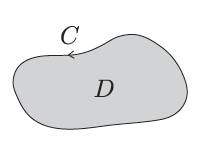
\includegraphics[height=25mm, width=35mm]{green.jpg}
 %\caption{キャプション。}
\end{wrapfigure}
 $D \subset \R^2$を$C$で囲まれる有界閉集合および, $C$の進行方向の左側に$D$があるとは右の図のようなことが成り立つことである
 
 
\begin{exa}
$C:\vec{p}(t)=(\cos t , \sin t) (0\leqq t \leqq 2\pi)$とし, $\R^2$上のベクトル場$V(x,y)=(x^2-y^2,-2xy)$とする. \\
線積分$ \int_{C}V(\vec{p}) d\vec{p} = \int_{C}(x^2-y^2)dx-2xydy$を求めよ.

\hspace{-11pt}(解.)普通に計算すると, 
\begin{align*}
\begin{split}
\int_{C}V(\vec{p}) d\vec{p}  
&= \int_{0}^{2\pi} \left \{(\cos^2 t - \sin^2 t)\drv{x}{t}-(2\sin t \cos t) \drv{y}{t} \right \} dt \\
&=\int_{0}^{2\pi} \left \{ -\cos^2 t \sin t + \sin^3 t -2\sin t \cos^2 t  \right\}dt
= \text{(計算略)}
= 0
\end{split}
\end{align*}

グリーンの定理を使う方法は以下のようになる.

$C$で囲まれた領域$D$とすると, $D$は原点中心の半径1の円である.
$V(x,y)=(u(x,y) , v(x,y))=(x^2-y^2,-2xy)$は$D$を含む開集合上で定義された$C^1$級ベクトル場である.\footnote{今回は$D$を含む開集合として$\R^2$が取れる.}
よってグリーンの定理の仮定を満たす.
$$
\pdrv{v}{x}=\pdrv{(-2xy)}{x}=-2y, \text{\,\,} \pdrv{u}{y}=\pdrv{(x^2-y^2)}{y}=-2y \text{\,\,であるため, }
$$
$$
\int_{C}(x^2-y^2)dx-2xydy =\iint_{D}\left(\pdrv{v}{x} - \pdrv{u}{y} \right)dxdy = \iint_{D}\left(-2y + 2y \right)dxdy =0.
$$
\end{exa}

\begin{exa}
$a,b$を正の数として, 楕円$D$を下で定める.
$$D = \left\{ (x,y) \in \R^2 : \frac{x^2}{a^2}+\frac{y^2}{b^2} \leqq 1 \right\}
=\left\{ (x,y) \in \R^2 :  -a \leqq x \leqq a, -b\sqrt{1-\frac{x^2}{a^2}} \leqq y \leqq b\sqrt{1-\frac{x^2}{a^2}} \right\}.
$$
$D$の面積$\Area(D)$を求めよ.

\hspace{-11pt}(解.)普通に計算すると, 
\begin{align*}
\begin{split}
\Area(D)=\int_{D}dxdy
= \int_{-a}^{a} \left( b\sqrt{1-\frac{x^2}{a^2}}-(-b)\sqrt{1-\frac{x^2}{a^2}}\right) dx =\int_{-a}^{a} 2 b\sqrt{1-\frac{x^2}{a^2}} dx =\text{(計算略)} = \pi ab.
\end{split}
\end{align*}

グリーンの定理を使うと以下の通りになる.
$C :\vec{p}(t) = (a \cos t, b \sin t) (0 \leqq t \leqq 2\pi)$と置けば,
楕円$D$は$C$で囲まれた領域となる.
よってグリーンの定理が使えて, $\drv{y}{t} = b \cos t$のため, 
$$
\Area(D)=\int_{C}xdy=\int_{0}^{2\pi} a \cos t \drv{y}{t} dt
= \int_{0}^{2\pi} ab \cos^2 t  dt = \pi ab.
$$
となる. (どちらが楽かは皆さんに委ねます.)
\end{exa}

 
\newpage

\begin{center}
{\Large 第14回. 面積分と体積分, 表面積と体積 \\ (川平先生の本, 第11・28章の内容)}
\end{center}

\begin{flushright}
 岩井雅崇, 2021/01/26
\end{flushright}

\section{はじめに}
第13回と第14回はベクトル解析の初歩(イントロ)に関する授業を行う.
授業準備のために, 以下の文献も参考した.
\begin{itemize}
\item 川平友規先生 解析学概論第三第四(ベクトル解析) available at \url{http://www.math.titech.ac.jp/~kawahira/courses/17W-kaiseki.html}
\end{itemize}
時々この文献を引用する.(引用する際は"川平先生のpdf"と呼ぶことにする.)


\section{曲線の長さ(復習)}
 \begin{tcolorbox}[
    colback = white,
    colframe = green!35!black,
    fonttitle = \bfseries,
    breakable = true]
    \begin{dfn}
$\R^2$内の滑らかな曲線$C: \vec{p}(t) = (x(t), y(t)) (a \leqq t \leqq b)$について. 曲線$C$の長さ$l(C)$を
$$
l(C) = \int_{a}^{b} \sqrt{\left( \drv{x}{t}\right)^2 + \left( \drv{y}{t}\right)^2}
=\int_{a}^{b} \left|\left| \drv{\vec{p}(t)}{t}\right|\right|dt
\text{と定義する.}
$$
 \end{dfn}
 \end{tcolorbox}
\section{面積分}

 \begin{tcolorbox}[
    colback = white,
    colframe = green!35!black,
    fonttitle = \bfseries,
    breakable = true]
    \begin{dfn}
$\vec{a}=(a_1,a_2,a_3), \vec{b}=(b_1,b_2,b_3) \in \R^3$とする.
\begin{itemize}
\item \underline{ベクトル$\vec{a}$の長さ$||\vec{a}||$}を$||\vec{a}||=\sqrt{a_{1}^{2} + a_{2}^{2}+a_{3}^{2}}$とする.
\item \underline{外積$\vec{a} \times \vec{b}$}を
$$
\vec{a} \times \vec{b} = (a_2b_3-a_3b_2, a_3b_1-a_1b_3, a_1b_2-a_2b_1) \text{\,\,とする.}
$$
\end{itemize}

 \end{dfn}
 \end{tcolorbox}
 
  \begin{exa}
 $\vec{a}=(1,0,0), \vec{b}=(1,2,0) \in \R^3$とする.
 
$||\vec{a}||=\sqrt{1^{2} + 0^{2}+0^{2}}=1$かつ, $||\vec{b}||=\sqrt{1^{2} + 2^{2}+0^{2}}=\sqrt{5}$である.

また, $\vec{a} \times \vec{b}=(0,0,2)$かつ, $\vec{b} \times \vec{a}=(0,0,-2)$である.
 \end{exa}
 
  \begin{tcolorbox}[
    colback = white,
    colframe = green!35!black,
    fonttitle = \bfseries,
    breakable = true]
    \begin{dfn}[川平先生のpdf 6章(プリント06)参照]
    \text{}
    
\begin{itemize}
\item \underline{$\Omega \subset \R^2$が閉領域}とは, ある領域$D$があって, $\Omega = D \cup \partial D$となること. (つまり$\Omega$が$D$と$D$の境界の和集合となること.)
\item $\Omega \subset \R^2$を閉領域とし, $x(s,t), y(s,t),z(s,t)$を$\Omega $上の連続関数とする.

 $$
\begin{array}{ccccc}
\vec{p}: &\Omega & \rightarrow & \R^3 & \\
&(s,t) & \longmapsto & ( x(s,t), y(s,t),z(s,t) )&
\end{array}
$$
という関数$\vec{p}(s,t)$を考える.
$$
S =\{\vec{p}(s,t) : (s,t) \in \Omega \}=\{(x(s,t), y(s,t),z(s,t) ) : (s,t) \in \Omega \}
$$
を$\R^3$内の曲面という.
\item $\R^3$内の曲面$S: \vec{p}(s,t) ((s,t) \in \Omega)$について, \underline{$S$が$\R^3$内の滑らかな曲面}であるとは, 次の二つの条件を満たすこと.
\begin{enumerate}
\item[条件1.] $x(s,t), y(s,t),z(s,t)$は$C^1$級.
\item[条件2.] $\pdrv{\vec{p}}{s} = \left( \pdrv{x}{s}, \pdrv{y}{s},\pdrv{z}{s} \right)$と
$\pdrv{\vec{p}}{t} = \left( \pdrv{x}{t}, \pdrv{y}{t},\pdrv{z}{t} \right)$が一次独立となる.
(つまり$\pdrv{\vec{p}}{s} \times \pdrv{\vec{p}}{t} \neq \vec{0}$となること.)
\end{enumerate}
\item $\R^3$内の滑らかな曲面$S: \vec{p}(s,t) ((s,t) \in \Omega)$について
$$\vec{n} = \frac{ \pdrv{\vec{p}}{s} \times \pdrv{\vec{p}}{t}}{  \left|\left|  \pdrv{\vec{p}}{s} \times \pdrv{\vec{p}}{t} \right|\right|} \text{を\underline{単位法線ベクトル}という.}$$
\end{itemize}


 \end{dfn}
 \end{tcolorbox}
 
 \begin{exa}
 \label{sphere}
 $\Omega = \{ (s,t) \in \R^2 : \sqrt{s^2+t^2} \leqq 1\}$とする.これは閉領域である.\footnote{$D= \{ (s,t) \in \R^2 : \sqrt{s^2+t^2} < 1\}$とすれば$\Omega = D \cup \partial D$となる.}
 
  $$
\begin{array}{ccccc}
\vec{p}: &\Omega & \rightarrow & \R^3 & \\
&(s,t) & \longmapsto & ( s, t, \sqrt{1-s^2-t^2} )&
\end{array}
\text{とすると, }
$$
$$
S=\{\vec{p}(s,t) : (s,t) \in \Omega \}=\{ (x,y,z) : 0 \leqq z, x^2+y^2+z^2=1 \}.
$$
つまり$S$は原点中心半径1の球の上半分の表面である.

また$\pdrv{\vec{p}}{s},\pdrv{\vec{p}}{t}$を計算すると, 
$$
\pdrv{\vec{p}}{s} = \left( 1, 0, \frac{-s}{\sqrt{1-s^2-t^2}}\right), \text{\,\,}
\pdrv{\vec{p}}{t} = \left( 0, 1,\frac{-t}{\sqrt{1-s^2-t^2}} \right) \text{であるため, }
$$
$$
\pdrv{\vec{p}}{s} \times \pdrv{\vec{p}}{t} 
=\left( \frac{s}{\sqrt{1-s^2-t^2}}, \frac{t}{\sqrt{1-s^2-t^2}}, 1\right).
$$
よって $\Omega$上で$\pdrv{\vec{p}}{s} \times \pdrv{\vec{p}}{t}  \neq \vec{0}$より$S$は滑らかな曲面である.

$$
 \left|\left|  \pdrv{\vec{p}}{s} \times \pdrv{\vec{p}}{t} \right|\right|
 =
 \sqrt{\frac{s^2}{1-s^2-t^2}    +    \frac{t^2}{1-s^2-t^2}   +1    }
 =
 \frac{1}{\sqrt{1-s^2-t^2}}  \text{\,\,であるため, }
 $$
 $$
\text{単位法線ベクトルは \,\,} \vec{n} = \frac{ \pdrv{\vec{p}}{s} \times \pdrv{\vec{p}}{t}}{  \left|\left|  \pdrv{\vec{p}}{s} \times \pdrv{\vec{p}}{t} \right|\right|}
 =
 (s,t,\sqrt{1-s^2-t^2})\text{\,\,となる.}
 $$
 \end{exa}

 \begin{tcolorbox}[
    colback = white,
    colframe = green!35!black,
    fonttitle = \bfseries,
    breakable = true]
    \begin{dfn}[川平先生のpdf 6章(プリント06)参照]
    \text{}
    
$\R^3$内の滑らかな曲面$S: \vec{p}(s,t)=(x(s,t), y(s,t),z(s,t) ) ((s,t) \in \Omega)$とし, $F(x,y,z)$を$S$を含む開集合上で定義された$C^1$級関数とする.
\underline{関数$F$の曲面$S$上での面積分}を
\begin{align*}
\begin{split}
\iint_{S}F(\vec{p}) dA
&=\iint_{\Omega}F(\vec{p}(s,t))\left|\left|  \pdrv{\vec{p}}{s} \times \pdrv{\vec{p}}{t} \right|\right|dsdt \\
&=\iint_{\Omega}F(x(s,t), y(s,t),z(s,t))\left|\left|  \pdrv{\vec{p}}{s} \times \pdrv{\vec{p}}{t} \right|\right|dsdt \text{と定義する.}
\end{split}
\end{align*}
特に\underline{$S$の表面積$\Area(S)$}を
$$
\Area(S)=\iint_{S}1 dA=\iint_{\Omega}\left|\left|  \pdrv{\vec{p}}{s} \times \pdrv{\vec{p}}{t} \right|\right|dsdt \text{と定義する.}
$$
 \end{dfn}
 \end{tcolorbox}

 \begin{exa}
 $S=\{\vec{p}(s,t) : (s,t) \in \Omega \}=\{ (x,y,z) : 0 \leqq z, x^2+y^2+z^2=1 \}$とするとき, $S$の表面積$\Area(S)=\iint_{S}dA$を求めよ.
 
 \hspace{-11pt}(解.)
 例\ref{sphere}から, $\Omega = \{ (s,t) \in \R^2 : \sqrt{s^2+t^2} \leqq 1\}$, $\vec{p}(s,t)=( s, t, \sqrt{1-s^2-t^2} )$とすると, 
$S=\{\vec{p}(s,t) : (s,t) \in \Omega \}$かつ
$ \left|\left|  \pdrv{\vec{p}}{s} \times \pdrv{\vec{p}}{t} \right|\right| = \frac{1}{\sqrt{1-s^2-t^2}}$である.

以上より, 
$$
\iint_{S}dA
=\iint_{\Omega}\left|\left|  \pdrv{\vec{p}}{s} \times \pdrv{\vec{p}}{t} \right|\right|dsdt
= \iint_{\Omega}\frac{1}{\sqrt{1-s^2-t^2}}dsdt
=\int_{0}^{2\pi} \int_{0}^{1} \frac{r}{\sqrt{1-r^2}} drd \theta
= 2\pi.
$$
よって, $S$(原点中心の半径1の球の表面の上半分)の表面積は $2\pi$である.


これにより原点中心の半径1の球の表面積は$2\pi \times 2 = 4\pi$である.

より一般に原点中心の半径$r>0$の球の表面積は$4\pi r^2$である.\footnote{厳密にやるなら$\Omega = \{ (s,t) \in \R^2 : \sqrt{s^2+t^2} \leqq r\}, \vec{p}(s,t)=( s, t, \sqrt{r^2-s^2-t^2} )$として同じ計算をする.}
 \end{exa}
 
  \begin{tcolorbox}[
    colback = white,
    colframe = green!35!black,
    fonttitle = \bfseries,
    breakable = true]
    \begin{thm}
$\Omega \subset \R^2$を閉領域とし, $f(s,t)$を$\Omega$上の非負の$C^1$級関数とする. \\
このとき
$S=\{ (s,t,f(s,t)) : (s,t) \in \Omega \}$
は滑らかな曲面となり, 曲面積$\Area(S)$は
$$
\Area(S) = \iint_{\Omega}\left( \sqrt{ \left( \pdrv{f}{s} \right)^2 + \left( \pdrv{f}{t} \right)^2+1 } \right)dsdt \text{\,\,で与えられる.}
$$
 \end{thm}
 \end{tcolorbox}
 
 \section{体積分}
  \begin{tcolorbox}[
    colback = white,
    colframe = green!35!black,
    fonttitle = \bfseries,
    breakable = true]
    \begin{dfn}[川平先生のpdf 11章(プリント11)参照]
    \text{}
    \begin{itemize}
    \item $\Omega \subset \R^2$が閉領域とし, $\phi_1, \phi_2$を$\phi_1(x,y) \leqq \phi_2(x,y)$となる$\Omega$上の連続関数とする.
    $$
    K=\{ (x,y,z) \in \R^3: (x,y) \in \Omega, \phi_1(x,y) \leqq z \leqq \phi_2(x,y) \}
    $$
    となる有界閉集合$K$を\underline{$z$方向の線領域}という.
    \item $K$を$z$方向の線領域とし, $F(x,y,z)$を$K$を含むある開集合上で定義された$C^1$級関数とする.
    \underline{$F(x,y,z)$の$K$上での体積分}を
    $$
    \iiint_{K}F(x,y,z)dxdydz = \iint_{\Omega} \left( \int_{\phi_1(x,y)}^{\phi_2(x,y)} F(x,y,z) dz \right)dxdy \text{\,\,と定義する.}
    $$
    
    特に\underline{$K$の体積$\vol(K)$}を
    $$
    \vol(K) = \iiint_{K}1dxdydz 
    =\iint_{\Omega} \left\{ \phi_2(x,y)-\phi_1(x,y) \right\}dxdy \text{と定義する.}
    $$
    \end{itemize}
     \end{dfn}
 \end{tcolorbox}
 
 \begin{exa}
$K = \{(x,y,z) \in \R^3 : 0 \leqq z, x^2+y^2+z^2 \leqq 1\}$とする.
$K$の体積$\vol(K)=\iiint_{K}1dxdydz $を求めよ.

\hspace{-11pt}(解.)
$\Omega= \{ (x,y) \in \R^2 : \sqrt{x^2+y^2} \leqq 1\}$とし, $\phi_1(x,y)=0, \phi_2(x,y)=\sqrt{1-x^2-y^2}$とすると, 
$K=\{ (x,y,z) \in \R^3: (x,y) \in \Omega, \phi_1(x,y) \leqq z \leqq \phi_2(x,y) \}$
となる.
よって, 
$$
\iiint_{K}1dxdydz 
=\iint_{\Omega} \sqrt{1-x^2-y^2}dxdy 
=\int_{0}^{2\pi} \int_{0}^{1}\left(\sqrt{1-r^2} \right)rdrd \theta
=\frac{2\pi}{3}
.$$
よって, $K$(原点中心の半径1の球の上半分)の体積は $\frac{2\pi}{3}$である.

これにより原点中心の半径1の球の体積は$\frac{2\pi}{3} \times 2 = \frac{4\pi}{3}$である.

より一般に原点中心の半径$r>0$の球の表面積は$\frac{4\pi r^3}{3}$である.\footnote{厳密にやるなら$\Omega = \{ (s,t) \in \R^2 : \sqrt{s^2+t^2} \leqq r\}$, $\phi_1(x,y)=-\sqrt{r^2-x^2-y^2}$, $\phi_2(x,y)=\sqrt{r^2-x^2-y^2}$として同じ計算をする.}

 \end{exa}
 
  \begin{exa}
  底面の半径$R>0$, 高さが$h>0$の円錐の体積を求めよ.
  
  \hspace{-11pt}(解.)
  小学校でやった知識を用いると, 
  $
  \text{(円錐の体積)} =  \text{(底面積)} \times \text{(高さ)} \times \frac{1}{3}
  $
  により, 体積は$\pi R^2 \times h \times \frac{1}{3} = \frac{\pi R^2 h}{3}$.
  
体積分を使うと次の通りである.
$\Omega= \{ (x,y) \in \R^2 : \sqrt{x^2+y^2} \leqq R\}$とすると, 円錐は
$$K=\left\{ (x,y,z) \in \R^3 : (x,y) \in \Omega, 0 \leqq z \leqq h \left(1- \frac{ \sqrt{x^2+y^2}}{R} \right) \right\}$$
という$z$方向の線領域$K$で表せられる.
以上より, 
$$
\vol(K)=
\iint_{\Omega} h \left(1- \frac{ \sqrt{x^2+y^2}}{R} \right)dxdy 
=
\int_{0}^{2\pi} \left(\int_{0}^{R}h \left(1- \frac{ r}{R} \right)rdr \right) d \theta
= \text{(計算略)}
=\frac{\pi R^2 h}{3}.
$$
よって 底面の半径$R>0$, 高さが$h>0$の円錐の体積は$\frac{\pi R^2 h}{3}$である.\footnote{小学校以来, なぜ$\frac{1}{3}$が出てくるのだろうと思った人も多いかもしれないが, これは積分による結果で出たものである. あともっと簡単な求め方もある.}
  \end{exa}



 \section{最後に}
第13回と第14回はベクトル解析の初歩(イントロ)に関する授業を行った. 
ベクトル解析は電磁気学などいろいろなところでお世話になる.(もしかしたら電磁気学や他の授業で詳しく学ぶかもしれません.)

ベクトル解析に関して, より詳しいことを学びたい人は
\begin{itemize}
\item 川平友規先生 解析学概論第三第四(ベクトル解析) available at \url{http://www.math.titech.ac.jp/~kawahira/courses/17W-kaiseki.html}
\end{itemize}
を参考にすると良い.
図などが綺麗に揃っててものすごく分かり易かった.

空間内の曲線や曲面に関しては
\begin{itemize}
\item 小林昭七 曲線と曲面の微分幾何 (裳華房)
\end{itemize}
が数学的に厳密で良いかもしれない.

私が10年前にベクトル解析を学んだときに使った本は
 \begin{itemize}
\item 渡辺正 ベクトル解析の基礎と応用 新数理ライブラリM5 (サイエンス社)
\end{itemize}
である. 結構ラフに書いていて, 数学的な厳密性抜きで学べた気がする.
もっともこの本に限らず, ネットで調べれば色々な本が見つかるので, 各自調べてみて吟味してください. 
\footnote{「スバラシク実力がつくと評判のベクトル解析キャンパス・ゼミ—大学の数学がこんなに分かる!単位なんて楽に取れる! (マセマ出版社)」という本もありますし... \\ もしかしたら私の授業の内容を「スバラシク実力がつくと評判の微分積分キャンパス・ゼミ—大学の数学がこんなに分かる!単位なんて楽に取れる!(マセマ出版社)」という本で勉強している人がいるかもしれません. もしこの本読んで私の授業の単位を楽に取れた場合はご一報ください. 以後の授業の参考にいたします.}

他にも"予備校のノリで学ぶ「大学の数学・物理」"チャンネルに再生リスト"ベクトル解析"や"電磁気学"があるので, ベクトル解析につまづいたらこちらで補うのもいいかもしれません.
(直感的にものすごくわかりやすかったです).

\end{document}
